% !TeX spellcheck = en_US
\section{Digital Video Streaming}
Digital video is the result of mapping real-world motion captured by a camera into the form of digital data.
Video consists of digital images (\emph{frames}), which are played back in sequence at a constant rate (\emph{frame rate}).
Independent frames consecutively played back are perceived as motion from around 14 to 18 \ac{FPS} on~\cite{Kandel2013}. 
Even for cases in which rapid changes are captured, the individual frames are not seen as independent images but as a smooth motion as soon as the frame rate reaches 60 \ac{FPS}~\cite{Kandel2013}.

In this work, the focus lies on two-dimensional video, which maps the three-dimensional world onto a two-dimensional plane.
Each of the video frames represents a raster image, in which each point contains visual information.
These points are called \emph{pixels}. 
The more pixels are available in a frame, the more visual information can be stored - usually allowing one to visualize more details.
The number of pixels in a video is determined by its \emph{resolution}, which is the width of a frame multiplied by its height in pixels.

Common video resolutions range from \ac{576p}, which represents analog television, over high-definition resolutions \ac{720p}, \ac{1080p} up to \ac{2160p}, also termed as ultra high definition.
A common, minimum representation of each pixel requires a bit depth of 8 bits per channel, where recently the evolution to 10 bits per channel has begun~\cite{Sullivan2012}.
It is evident that an encoding of each pixel in each video frame would cause an enormous size of a video.
For example, for one second of \ac{720p} video at a frame rate of 30 \ac{FPS} the resulting video would be of a size of approximately 79.1 \unit{MB}.

Particularly for high resolutions, areas in a digital frame may have very similar structures and colors.
Instead of describing these areas multiple times, a significant data size reduction can be achieved by describing redundant information only once.
This step, which compresses the digital video is termed as video encoding.
As this cannot only be applied to a single video frame, a compression can be extended to leverage redundancy between video frames.
If areas in a single or different video frames are detected with similar characteristics, they need to be encoded only once.
Note that for this thesis video encoding is solely discussed for compression reasons.

Prominent and widely applied video codecs - software or hardware which can compress and uncompress digital video - are H.264/\ac{AVC}~\cite{Wiegand2003} and H.265/\ac{HEVC}~\cite{Sullivan2012}.
These codecs determine the level of compression and specify how many bits are required per second of digital video, the \emph{bit rate}\footnote{In this thesis, \emph{bit rate} describes a property of the video and not of the channel.}.
Besides many codec-specific features, they achieve this compression by quantization.

The concepts of frame rate, resolution, and bit rate are essential for the understanding of this thesis, as they describe the dimensions that allow adaptation\footnote{Recent codecs additionally allow to adapt the bit depth and the color gamut~\protect\cite{Sullivan2012}.}.

Video streaming refers to the download of a digital video over a communication network and the in-parallel video playback before the download is completed.
It is a delivery mode for digital video.
A device capable of streaming video must be able to receive, decode, and render small parts of a video - so-called chunks.
Also, it needs to ensure that the video chunks arrive in time.
Thus, the network throughput should be equal or higher than the bit rate of the video.
To compensate for small variations in the achieved throughput, streaming devices leverage the concept of a \emph{playback buffer}, which stores video chunks before playback.
Download rates higher than the video bit rate allow for filling the buffer faster than chunks being consumed by the video player.

Video streams can be distinguished by timing deadlines of the stream: \ac{VoD} and live video~\cite{Liu2003}.
Whereas \ac{VoD} represents completely encoded video files - which can be requested and consumed at any time - the live video is distributed instantly while the content is being recorded and encoded.
Well-known \ac{VoD} services include the \ac{UGV} platform YouTube\footnote{https://youtube.com; Visited on: 09/14/2016}, as well as the video streaming portals of Netflix\footnote{https://netflix.com; Visited on: 09/14/2016} and Amazon Instant Video\footnote{https://amazon.com; Visited on: 09/14/2016}.

In contrast to \ac{VoD}, live video streaming describes the real-time production, delivery and consumption of video. 
All these steps are realized during an event is happening.
Environmental and legal conditions also affect what is perceived as a live video.
For example, a live video broadcast from United States \ac{TV} stations can be delayed between five seconds and five minutes\footnote{http://news.bbc.co.uk/2/hi/entertainment/3478467.stm; Visited on: 09/14/2016}, due to artificial delays invoked by stations to avoid fines for broadcasting explicit content.
Still, in comparison to \ac{VoD} the technical possibilities for distributing, caching and preloading of live video are rather limited. 
\section{Application Scenario}
The scenario described in this thesis assumes an end-to-end transmission of a live video recorded on a mobile device using an access network technology, routing it through the core of a fixed network to a remote viewing device, which receives the stream (see Figure~\ref{fig:205_relatedworkmbsstreaming}).
In this scenario, the upload and distribution of a live video stream are decoupled by a server which receives the provided stream and prepares it for distribution.
\begin{figure}[tbh]
\centering
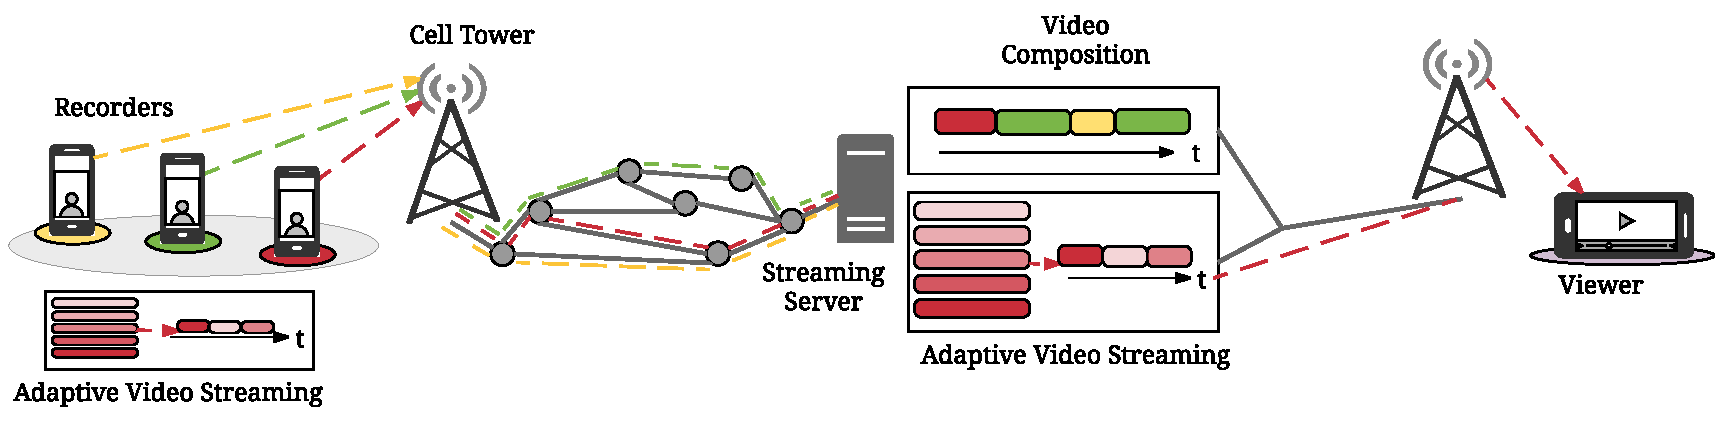
\includegraphics[width=\linewidth]{gfx/200_Background/RelatedWork_MBS_Streaming}
\caption[Content Adaptation in the live video upload scenario]{Options for content adaptation in the scenario introduced in Figure 1.}
\label{fig:205_relatedworkmbsstreaming}
\end{figure}

The streaming server does not only consume a single video but can potentially process multiple, in-parallel recorded streams at the same time.
It acts as a decoupling element of the video upload and its distribution.
Preparation for the distribution on the server can be transcoding of different versions of a video for adaptive video streaming (see Section~\ref{sec:205_video_adaptation}) or video composition (see Section~\ref{sec:205_video_composition}).
\subsection{Smart Mobile Devices}
The devices discussed in this thesis are assumed to be smart mobile devices.
They incorporate four features: 1) they are capable of real-time capturing, encoding, decoding, and rendering of digital video, 2) they have additional sensors that describe the geographic position and capture the environmental conditions, i.e., the context, 3) they can be connected to at least one wireless communication network, 4) they are battery powered and can be freely moved.
\subsubsection{Video Recording}
Smart mobile devices are also termed recording devices when their functionality of capturing a real-world scene as a digital video is in focus.
Video recording is achieved by using the camera sensors in a recording device.
In conjunction with a microphone, visual information and audio can be stored in a single digital video stream.
This thesis focuses on the visual part of a digital video.

The recording device generates a two-dimensional representation of a scene.
What a camera sensor captures is very much dependent on its technical capabilities: the technical design of the sensor, its resolution, angle of view, and focal length.
For simplification reasons, the result of these different attributes is described as the \emph{\ac{FoV}}~\cite{Ay2008}.
The \ac{FoV} describes what is being captured in a scene and encoded in a digital video frame.

\begin{figure}[tbh]
\centering
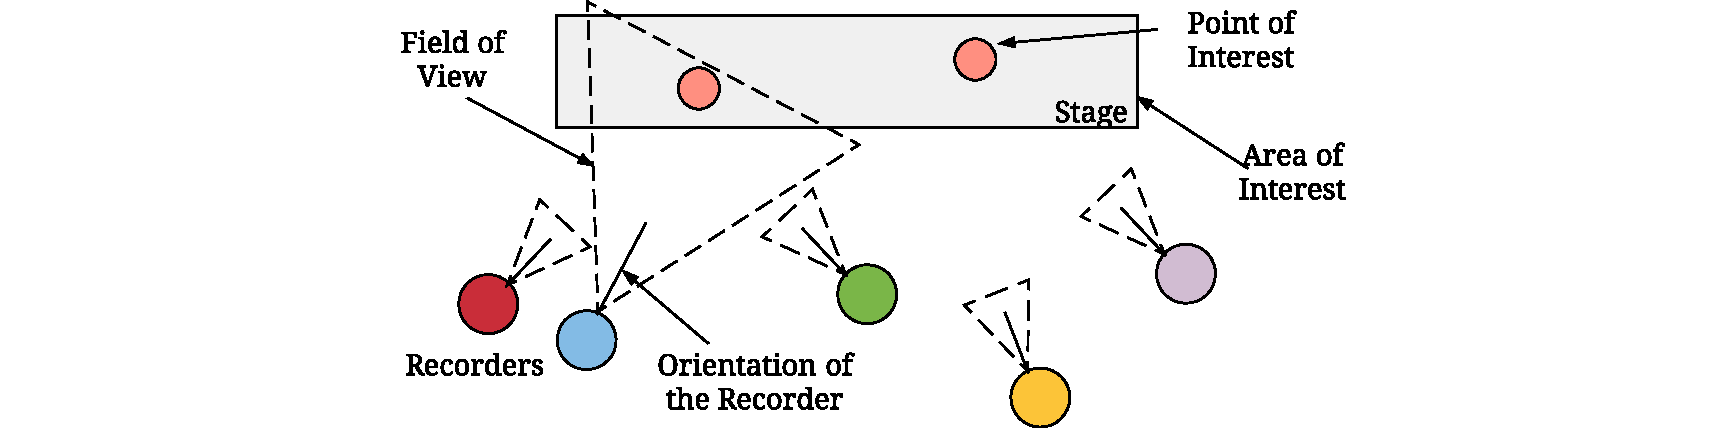
\includegraphics[width=\linewidth]{gfx/200_Background/RelatedWork_ROI}
\caption{Illustration of the concepts RoI, AoI and FoV.}
\label{fig:205_relatedworkroi}
\end{figure}
In a video frame, the \emph{\ac{RoI}} captures what is of specific interest for the recorder.
The \ac{RoI} represents a region in the video frame, which captures the visual and semantic information of a scene that is needed for understanding the captured content.
Mapping the \ac{RoI} of a recorded video to the real world allows retrieving coordinates, e.g., in the format of the \ac{GPS} as longitude, latitude, and altitude.
For simplification reasons only the latitude and longitude values of a recorded scene are used to describe the \emph{\ac{AoI}}. 
Within an \ac{AoI} different \emph{\acfp{PoI}} can be positioned, which depict marks of interest, e.g., persons.
The three concepts of \ac{FoV}, \ac{RoI} and \ac{AoI} are illustrated in Figure~\ref{fig:205_relatedworkroi}.
The concepts of  \ac{FoV}, \ac{RoI} and \ac{AoI} are not only required when different devices collaboratively record the same scene, but they as well as many algorithms proposed in this thesis can be applied to independent \ac{UGV} streams.
\subsubsection{Video Playback}
Each smart mobile device is capable of not only capturing live video but also receiving it.
These devices leverage electronic circuit-based decoders for uncompressing digital video, and a media playback software (i.e., a video player) for rendering on the display.
The playback experience is very much dependent on the context while watching a video stream.
Section~\ref{sec:250_background_content_aware_delivery} discusses which influence the video stream, the encoded content and content adaptations have on the quality of a video playback.

\subsubsection{Sensors}
To capture not only video and sound, smart mobile devices have also auxiliary sensors to understand the environment and context of a video recording or playback session.
A reasonable classification of the different sensors available in today's smartphones is found in the documentation of the Android \ac{OS}.
Available sensors are classified into motion, environmental, and position sensors\footnote{https://developer.android.com/guide/topics/sensors/sensors\_overview.html; Visited on: 09/14/2016}.

\emph{Motion sensors} measure forces applied to the smart mobile device, and differ depending on the type of force. 
What all of these sensors have in common is that they represent the forces in a tri-axial form (x,y,z).
Accelerometers measure current acceleration forces in $\unit{\frac{m}{s^2}}$ on each of the three physical axes.
Gravity sensors are affected by the current gravity force without any device motion in all three physical axes ([$\unit{\frac{m}{s^2}}$]).
A gyroscope measures the rotation applied to a device in each of its axes in $\unit{\frac{rad}{s}}$. 
An example of its use is to measure the orientation of the device.

\emph{Environmental sensors} measure parameters to describe the context around a device. 
Examples of these sensors include ambient air temperature and pressure, humidity, and probably most famous the illumination sensor, which is used to adapt the screen brightness. 
A device's camera and microphone are also classified as environmental sensors.

Finally, \emph{position sensors} describe the physical position of the device in longitude, latitude, and altitude.
The most prominent example is \ac{GPS}.
The geographic orientation of a device is the fusion of the gravity sensor and a magnetometer to measure the geomagnetic field.
Compass readings provided by some location providers are thus from a virtual sensor, which fuses gravity and magnetometer measurements. 
\subsubsection{Network Access}
Communication networks are used to allow different devices to communicate with each other.
A communication network uses a single technology to interconnect autonomous devices to allow them to exchange data~\cite{tanenbaum2003computer}.
A network can be part of other networks, so-called networks-of-networks, where the most prominent is the Internet~\cite{tanenbaum2003computer}.
Here, the single technology used by all devices is the \ac{IP}, which allows the addressing of devices and the routing of messages.
Thus, \ac{IP} offers a rich set of functionalities but by itself is not sufficient to enable communication between different devices.
The concept of protocols reduces the complexity in communication networks, which encapsulate well-defined functionality.
Protocols are classified to belong to specific layers in a protocol stack to illustrate how they communicate.
Protocols on different layers do usually not know of each other.
On the same layer, it is assumed that two communicating devices use the same or at least compatible protocols.

Communication networks can be further classified as wired or wireless communication networks.
The latter use wireless connections between communicating devices. Usually, at least one participant of the wireless connection is a mobile device.
This thesis follows the \ac{ISO}/\ac{OSI} protocol stack (see~\cite{tanenbaum2003computer}).
We mainly discuss innovations on the application layer of the stack.
Due to the layered concept of the stack, the contributions of this thesis are not aware of the underlying network.
\ac{IP} and upper layer protocols hide the underlying technology from the application layer, making the proposed contributions independent of the used technology.
A simple classification of wireless communication networks into cellular networks and \acp{WLAN} is used.
For each of the categories, a prominent example is used, such as \ac{LTE}~\cite{Astely2009} for cellular networks and \ac{IEEE} 802.11~\cite{tanenbaum2003computer} for \acp{WLAN}.
For this thesis, it is assumed that two metrics can be easily calculated on the application layer for describing the performance of the communication network: the end-to-end application-layer \emph{throughput} and \emph{delay}. 
For this thesis, the \emph{delay} describes the total time from sending a message until it is completely received.
The \emph{throughput} depicts the actual transmission speed of a channel.
In contrast, we understand the bandwidth as a description of the theoretically, maximum amount of data that can be transmitted over a channel per time unit.
\subsubsection{Mobility}
The mobility of the smart mobile devices induces challenges for both video recording and playback.
First, to achieve mobility the devices are battery powered -  this limits their maximum operating time.
The investigation energy consumption of video recording, uploading and streaming is outside of the focus of this work.

Also, mobility affects the connection to a computer network, the reliability of individual hosts, the throughput, and the delay.
In wireless networks, mobility can mean that the communication range of a stationary cell tower or access point is left so that connections are lost, and streaming or uploading of video is interrupted.
An assumption in this thesis is that a detection of the device position and its mobility, i.e., at which speed it moves into which direction, is provided by a location provider on the smart mobile device.
\subsection{Content Adaptation}
The core of this thesis is the investigation of different types of content adaptation to achieve a reliable, high-quality streaming from mobile devices to mobile devices.
Content adaptation is a concept already used in the web for the delivery of websites.
It is the process to transform a page based on the capabilities of the device or a communication network, as well as to the user and his experience or preferences~\cite{Rabin10}.

Similar concepts are proposed for the creation, transmission and consumption of live video streams.
In this work, two types of content adaptation are discussed: the adaptive video streaming and video composition.
Both concepts can be placed on the recorders, the servers and the receiving video streaming clients (see Figure~\ref{fig:205_relatedworkmbsstreaming}).
The conceptual difference of the two content adaptation types is illustrated in Figure~\ref{fig:205_relatedworkcontentadaptation}.
Whereas adaptive video streaming provides adaptation within a video, video composition leverages adaptation between videos.
\begin{figure}[tbh]
	\centering
	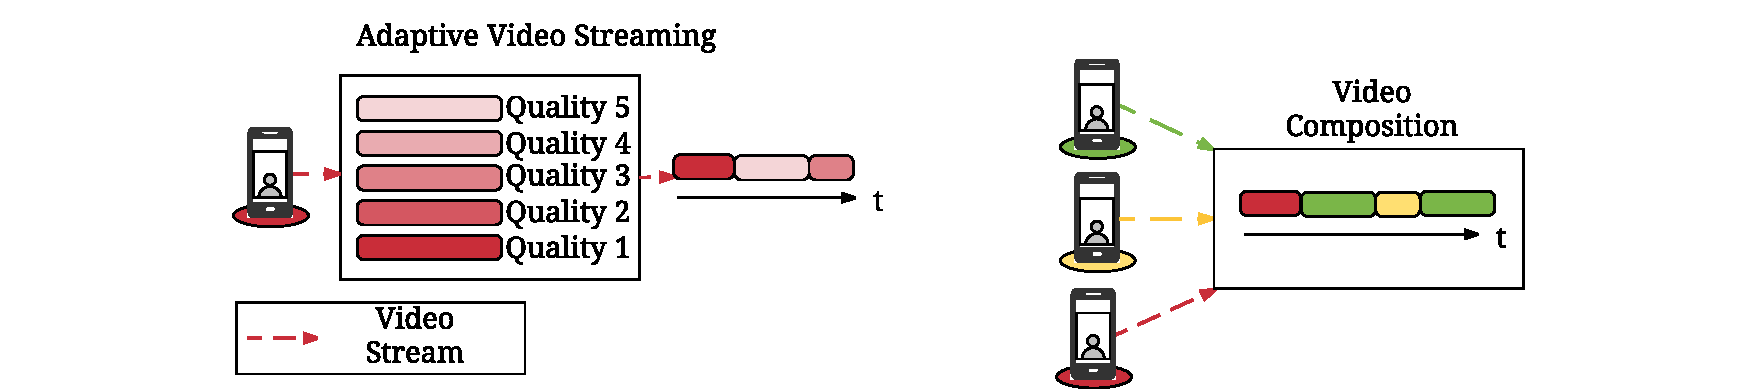
\includegraphics[width=\linewidth]{gfx/200_Background/RelatedWork_ContentAdaptation}
	\caption[Adaptive video streaming versus video composition]{Conceptual difference of adaptive video streaming and video composition.}
	\label{fig:205_relatedworkcontentadaptation}
\end{figure}
\subsubsection{Adaptive Video Streaming}
\label{sec:205_video_adaptation}
Adaptive video streaming is usually applied to the delivery of a digital video to compensate variations in the network conditions, mostly the throughput, during playback~\cite{DeCicco2010}.
A digital video is made available in different versions, where each version is different regarding the average bit rate.
The video could also change in the other dimensions such as the frame rate or the resolution.

Adaptive video streaming allows devices to switch between different versions of a video, e.g., for adjusting the video stream bit rate to network conditions.
Adaptive video streaming can be supported by the video encoding. 
Two categories of video encodings are discussed: the \acf{SVLC} and \acf{MVLC}.
\paragraph{\acf{SVLC}}
The advantage of \ac{SVLC} is the wide support regarding hardware encoders and decoders and software video players.
When using \ac{SVLC} each video version is a single, independent decodable video file.
Currently, all of the supported video encodings on mobile phones are based on \ac{SVLC}, such as H.264/\ac{AVC}, VP8, H.265/\ac{HEVC} or VP9~\cite{Feller2011,Mukherjee2013,Sullivan2012,Wiegand2003}.
\paragraph{\acf{MVLC}}
\ac{MVLC} supports adaptive video streaming by organizing the video representations as interdependent layers.
Each layer encodes the delta of information to the next lower layer.
It reduces the redundancy between video representations to a minimum.
Additional data is needed to organize the interdependencies.
The main advantage of using \ac{MVLC} for many streaming applications is solely a reduced storage requirement on the streaming server.

Some of the latest \ac{SVLC} approaches have multi-layered variants, such as H.264/\ac{SVC}~\cite{Schwarz2007} and H.265/\ac{SHVC}~\cite{Boyce2016}.
Besides its complexity in decoding, it has been shown that the imagined benefits are very limited in practice.
The overhead using \ac{MVLC} is higher than the saved data traffic in comparison to \ac{SVLC}, when more than three layers are encoded~\cite{Grafl2013,Wang2013}. 

Note that multiple description coding is a related approach to \ac{MVLC} which has been omitted due to lack of support on today's mobile or stationary devices~\cite{Setton2008}.
Details on the current state of adaptive video streaming systems are given in Section~\ref{sec:250_background_content_aware_delivery}.
\subsubsection{Video Composition}
\label{sec:205_video_composition}
Whereas adaptive video streaming leverages different versions of the same content, video composition combines segments of different videos to create a new video stream.
In the case of a given application scenario, the content that can be selected is represented by the recording devices.
Video composition can select which view to show at a given time from all the available video recording sources.

The concept of video composition, as well as influencing factors like its effect on the perceived quality, are discussed in Section~\ref{sec:240_videocomposition}.
